\chapter{Ouroboros Genesis}
\label{genesis}

\section{Introduction}

\subsection{Chain length versus chain density}

The purpose of chain selection to resolve temporary forks that arise from the
normal operation of the protocol (such as when there are multiple leaders in a
single slot), and---importantly---to distinguish honest chains from chains
forged by malicious nodes. It is not a priori clear why choosing longer chains
over shorter chains would help distinguish malicious chains from honest chains:
why would an honest chain be longer?

By assumption, the malicious nodes in the system together have less stake than
the honest nodes; security of the system as a whole critically depends on the
presence of this honest majority. Since the leadership schedule is determined
based on stake, this means that we expect the \emph{proportion} of slots filled
by malicious nodes to be smaller than the proportion of slots filled by honest
nodes. Similarly, we would expect a chain forged by a malicious node to be
\emph{less dense} than an honest chain, forged by the honest nodes in the
system: the malicious node has less stake, and so must necessarily leave many
slots empty (assuming they can't cooperate with honest nodes).

When all nodes in the system are up to date, they will all share the shame
chain, except for blocks near the tips of those chains. Moreover, blocks whose
slot number is ahead of the wall clock are considered invalid. This means that
the only way for one chain to be longer than another is by having more filled
slot between the tip of the shared prefix and ``now'': in other words, they
must be \emph{denser}.
%
\begin{center}
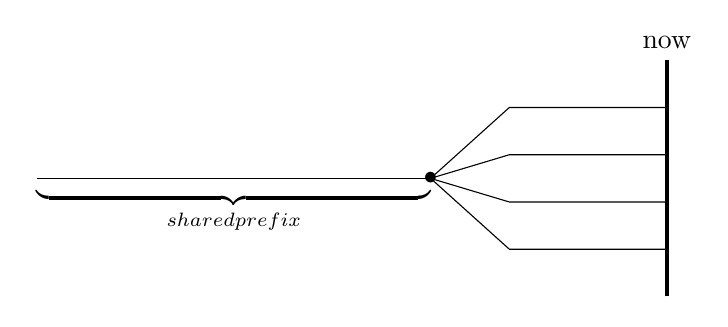
\begin{tikzpicture}
\draw (0,0) -- (5,0) coordinate(branch) node{$\bullet$} node[pos=0.5,below]{$\underbrace{\hspace{5cm}}_\text{shared prefix}$};
\draw (branch) -- ++(1,  0.9) -- ++(2,0);
\draw (branch) -- ++(1,  0.3) -- ++(2,0);
\draw (branch) -- ++(1, -0.3) -- ++(2,0);
\draw (branch) -- ++(1, -0.9) -- ++(2,0);
\draw [ultra thick] (8,-1.5) -- (8,1.5) node[above]{now};
\end{tikzpicture}
\end{center}
%
Conversely, the density on the fragment of a chain is only meaningful if that
fragment is long enough. Since the leadership election is a probabilistic
process, we only expect fragments to contain more slots signed by honest nodes
\emph{on average}, and we can only draw conclusions from density on long enough
fragments.

\subsection{Speculative mode}

Chain selection so far has been running in what we might call a ``speculative``
mode: when we see a new chain, we compare it to our current chain, and if we
prefer it (if is longer), we adopt it. This is speculative in the sense that
if we later see a second chain, we can change our mind about adopting the
first and adopt the second if that second chain is preferred over the first.

The Praos chain selection rule (choose the longest chain) was explicitly
designed for a context in which all nodes in the network are present from the
very beginning and are always online. The Praos security analysis
\cite{cryptoeprint:2017:573} essentially shows that when the honest nodes in the
system are all following this protocol, they will end up with a common prefix,
differing only in the most recent $k$ blocks. This means that nodes never need
to roll back past the tip of that common prefix; indeed, they \emph{should} not
roll back past that point, as this might mean they might adopt a chain forged by
a malicious node which is trying to trick them into believing some kind of
alternative history. This is the reason for the ``no rollback more than $k$
blocks'' rule in the Praos chain selection rule, as well as the justification
for the fact that much of the consensus layer is designed around the assumption
that there exists a maximum rollback distance.

In reality of course new nodes join the system all the time. This is problematic
for at least two reasons. First, within the consensus layer we don't see a
candidate chain's \emph{true} length; the length of a candidate we see depends
on how much of that candidate's chain we have downloaded\footnote{Nodes do
report their ``true length'', but since we have no way of verifying this
information until we have seen the entire chain, we can make no use of this
information for the purpose of chain selection.}. Of course, defining chain
selection in terms of chain length, where our \emph{perceived} chain length
depends on what we decide to download, is rather circular indeed.

But actually the problem is more fundamental than that. Recall that chain
selection is running in speculative mode: we consider chains as we see them,
possibly changing our mind later by adopting a different chain. If a new node
sees a chain constructed by a malicious node and adopts it, \emph{it might be
stuck}: it is not difficult for an attacker to construct a chain that is longer
than $k$ blocks long, and so once a node adopts such a chain, it will not be
able to switch to the honest chain anymore, as this would involve a roll back
of more than $k$ blocks.

\subsection{Genesis rule}

Any node with non-zero stake can easily construct chains of arbitrary length,
but such chains will necessarily be sparse. Indeed, as we argued above,
chains constructed by malicious nodes cannot be denser (on a sufficiently
long fragment) than the honest chain.

The \emph{Genesis chain selection rule}, designed to cope with new nodes joining
the network, therefore compares chains on density whenever possible, defaulting
to comparing chain length only if the aren't enough blocks to do a meaningful
density comparison. The size of this ``density window'' is a parameter to the
rule known as $s$, although we can set $s = \frac{1}{4}(k / f)$.

\begin{definition}[Genesis rule]
\label{genesis:rule}
A candidate chain is preferred over our current chain if

\begin{itemize}
\item The intersection between the candidate chain and our chain is \textbf{at
least $s$ slots} back from the tip of our chain, and the candidate chain is
\textbf{denser} in a window of $s$ slots at the intersection, or

\item The intersection between the candidate chain and our chain is \textbf{less
than $s$ slots} back from the tip of our chain, and the candidate chain is
strictly \textbf{longer} than our chain.
\end{itemize}

\end{definition}

\subsection{Conservative mode}

The rule as defined in \cref{genesis:rule} is problematic for consensus:
\emph{it no longer imposes a maximum rollback}. We depend on this maximum
rollback in many ways (todo: reference), and we will want to \emph{continue}
to be depend on it. We solve it by switching from the default
speculative chain selection mode to a \emph{conservative} chain selection mode.
We will see the details of how this mode works later in this chapter, but
the intuition is rather than considering and possibly adopting chains as we
encounter them, we instead wait, collecting information, until we have enough
information that we can decide which block to adopt next, \emph{knowing we will
never have to change about mind}: we will never need to roll back that block.

The security analysis of the genesis chain selection rule includes a theorem
\cite[Theorem 2]{cryptoeprint:2018:378} that says that it is still true that
when nodes are up to date they will never need to roll back more than $k$
blocks. We can use this theorem to justify switching from the conservative
mode back to the speculative mode. Since blocks ahead of the wall clock are
considered invalid, we can use the current slot number (according to the
wallclock) to estimate if we are within $k$ blocks from the longest chain
in the network. This remains an estimate because we might not know the
density of that chain. At one extreme, we might assume that the density is
1, and so only switch to speculative mode when we are within $k$ \emph{blocks}
from the wall clock. At the other extreme, we might assume that the density is
precisely the theoretical ideal $f$, at the cost of switching to speculative
mode too early and being unable to roll back when we really should. Probably
the actual switch-over point should lie somewhere between these two extremes.

The switch over point does not change the chain selection rule itself: even when
we are in speculative mode, we will still apply the genesis rule as defined in
\cref{genesis:rule}, comparing density or length depending on the intersection
point; we will merely use Theorem 2 of the genesis security analysis to justify
imposing the standard maximum rollback of $k$ blocks.


\pagebreak
\debugsep{OLD}

\section{The Genesis Chain Selection Rule}

\subsection{Introduction}

The genesis rule is an improved chain selection rule, designed to help new nodes
safely join the network even in the presence of potential long range attacks
\cite{cryptoeprint:2018:378}. From the point of view of the consensus layer,
however, the \emph{why} is less relevant than the \emph{what} and the
\emph{how}. Let's start with the \emph{what}. The genesis chain selection
rule defined as follows.

\begin{definition}[Genesis chain selection rule]
\label{genesis:originalrule}
A candidate chain is preferred over our current chain if

\begin{itemize}
\item The intersection between the candidate chain and our chain is \textbf{no
more than $k$} blocks back, and the candidate chain is strictly \textbf{longer}
than our chain.

\item If the intersection \emph{is} \textbf{more than $k$} blocks back, and the
candidate chain is \textbf{denser} (contains more blocks) than our chain in
a region of $s$ slots starting at the intersection.
\end{itemize}
\end{definition}

Condition (B) of this definition is what sets the genesis rule apart from the
Praos chain selection rule.\footnote{The \lstinline!TPraos! chain selection rule
of the Shelley ledger may additionally prefer candidate chains of equal length
under certain circumstances, see \cref{todo}.} The intuition is that an attacker
will have less stake than the majority (if this is not true, the chain is no
longer secure), and therefore if they try to construct an alternative history,
they can only produce a chain that is less dense than the real chain.

It is important that we compare density only \emph{at the intersection point}.
An example will make this obvious. Suppose the chain is growing normally,
then a malicious node with some stake intentionally skips their slot, after
which the chain continues to grow again:
%
\begin{center}
\begin{tikzpicture}
\draw
       (0,0) node{$\bullet$}
  -- ++(1,0) node{$\bullet$}
  -- ++(1,0) node{$\bullet$}
  -- ++(1,0) node{$\bullet$}
  -- ++(1,0) node[above]{$\times$}
  -- ++(1,0) node{$\bullet$}
  -- ++(1,0) node{$\bullet$}
  -- ++(1,0) node{$\bullet$};
\end{tikzpicture}
\end{center}
%
It is now trivial for an attacker to create an alternative chain that
\emph{does} have a block in that slot; if other nodes switch to the denser chain
the moment they see a window of $s$ slots that is denser, they would adopt the
attacker's chain; after all, it has one more block in the window than the real
chain does:
%
\begin{center}
\begin{tikzpicture}
\draw
       (0,0) node{$\bullet$}
  -- ++(1,0) node{$\bullet$} coordinate(s-anchor)
  -- ++(1,0) node{$\bullet$}
  -- ++(1,0) node{$\bullet$} coordinate(branch)
  -- ++(1,0) node[above]{$\times$}
  -- ++(1,0) node{$\bullet$}
  -- ++(1,0) node{$\bullet$}
  -- ++(1,0) node{$\bullet$};
\draw
       (branch)
  -- ++(1, -1) node{$\bullet$}
  -- ++(3,  0) node{$\bullet$};
\draw [dashed]
     (s-anchor)
  -- ++(0,1)
  -- ++(3.5,0)
  -- ++(0,-2.5)
  -- ++(-3.5,0) node[below, pos=0.5]{$\underbrace{\hspace{3.5cm}}_{\text{$s$ slots}}$}
  -- cycle;
\end{tikzpicture}
\end{center}
%
Instead, we must wait until we make such a comparison until we have reached
the intersection point:
%
\begin{center}
\begin{tikzpicture}
\draw
       (0,0) node{$\bullet$}
  -- ++(1,0) node{$\bullet$}
  -- ++(1,0) node{$\bullet$}
  -- ++(1,0) node{$\bullet$} coordinate(branch)
  -- ++(1,0) node[above]{$\times$}
  -- ++(1,0) node{$\bullet$}
  -- ++(1,0) node{$\bullet$}
  -- ++(1,0) node{$\bullet$};
\draw
       (branch)
  -- ++(1, -1) node{$\bullet$}
  -- ++(3,  0) node{$\bullet$};
\draw [dashed]
     (branch)
  -- ++(0,1)
  -- ++(3.5,0)
  -- ++(0,-2.5)
  -- ++(-3.5,0) node[below, pos=0.5]{$\underbrace{\hspace{3.5cm}}_{\text{$s$ slots}}$}
  -- cycle;
\end{tikzpicture}
\end{center}
%
Since the attacker does not have sufficient stake, if we \emph{now} compare the
attacker's chain to the real chain, we will find that the attacker's chain is
less dense and nodes will therefore not select it. If the attacker creates
another fork earlier on the chain, then we will resolve that fork
when we encounter it using a window of $s$ slots \emph{anchored at that fork},
and then later resolve the second fork using a \emph{different} window of
$s$ slots, anchored at the second fork:
%
\begin{center}
\begin{tikzpicture}
\draw
       (0,0) node{$\bullet$}
  -- ++(1,0) node{$\bullet$} coordinate(s-anchor)
  -- ++(1,0) node{$\bullet$}
  -- ++(1,0) node{$\bullet$} coordinate(branch)
  -- ++(1,0) node[above]{$\times$}
  -- ++(1,0) node{$\bullet$}
  -- ++(1,0) node{$\bullet$}
  -- ++(1,0) node{$\bullet$};
\draw
       (branch)
  -- ++(1, -1) node{$\bullet$}
  -- ++(3,  0) node{$\bullet$};
\draw
       (s-anchor)
  -- ++(1, -1) node{$\bullet$};
\draw [dashed]
     (s-anchor)
  -- ++(0,1)
  -- ++(3.5,0)
  -- ++(0,-2.5)
  -- ++(-3.5,0) node[below, pos=0.5]{$\underbrace{\hspace{3.5cm}}_{\text{$s$ slots}}$}
  -- cycle;
\draw [dotted]
     (branch) ++ (0, 0.1)
  -- ++(0,1)
  -- ++(3.5,0)
  -- ++(0,-2.5)
  -- ++(-3.5,0)
  -- cycle;
\end{tikzpicture}
\end{center}

\subsection{Alternative Formulation}

As phrased in \cref{genesis:originalrule}, the genesis chain selection rule has
a weird quirk. Consider the following situation, where we have two chains $C_1$
and $C_2$; $C_1$ is denser than $C_2$ at the intersection with $C_2$, but $C_2$
is longer:

\begin{center}
\begin{tikzpicture}
\path (0, 0) coordinate (tip) node{$\bullet$};
\draw (tip) -- ++(1.0,  0.5) -- ++(2.5, 0) coordinate(C1) node[right]{$C_1$};
\draw (tip) -- ++(1.0, -0.5) -- ++(3.5, 0) coordinate(C2) node[right]{$C_2$};
\draw [red, very thick] (tip) -- ++(1.0,  0.5) -- ++(2.0, 0);
\draw [dashed]
     (tip)
  -- ++(0, 0.75)
  -- ++(3, 0)
  -- ++(0, -1.5)
  -- ++(-3, 0) node[pos=0.5, below]{$\underbrace{\hspace{3cm}}_{\text{$s$ slots}}$}
  -- cycle;
\path (tip) -- (C1) node[pos=0.5, above=0.5cm]{$\overbrace{\hspace{3.5cm}}^{\text{fewer than $k$ blocks}}$};
\path (tip) -- (C2) node[pos=0.5, below=1.1cm]{$\underbrace{\hspace{4.5cm}}_{\text{more than $k$ blocks}}$};
\draw (tip) + (-3,0) node{$\bullet$} -- (tip);
\end{tikzpicture}
\end{center}

If our current chain is $C_1$, then the intersection point with $C_2$ is less
than $k$ blocks back, so condition (A) of the rule applies and we prefer $C_2$,
because $C_2$ is longer. But if our current chain is $C_2$, then the
intersection point with $C_1$ is \emph{more} than $k$ blocks back, and so
condition (B) of the rule applies, and we prefer $A$, because it is denser!

The rule as formulated in the paper (reproduced here in
\cref{genesis:maxvalid-bg}) does not suffer from this ``flip-flop'' behaviour,
but only because it considers chains strictly in order. If the list of chains
$\mathcal{N} = \{ C_1, C_2 \}$, we end up choosing $C_2$, and if that list is
$\mathcal{N} = \{ C_2, C_1 \}$, we end up choosing $C_1$.

The following alternative formulation of the genesis rule [Badertscher, personal
communication] avoids this problem. As we shall see (todo\todo{TODO}:
reference), it also suits our needs better:

\pagebreak

\begin{definition}[Alternative genesis rule]
\label{genesis:originalrule}
A candidate chain is preferred over our current chain if

\begin{itemize}
\item The intersection between the candidate chain and our chain is
\textbf{at least $s$ slots} back, and the candidate chain is denser in a window
of $s$ slots at the intersection, or

\item The intersection between the candidate chain and our chain is \textbf{less
than $s$ slots back and no more than $k$ blocks back}\footnote{This is
extremely unlikely to happen in $s$ slots.}, and the candidate chain is strictly
\textbf{longer} than our chain.
\end{itemize}

\end{definition}

Whichever variant we use however, it is clear that this rule breaks a bunch of
fundamental assumptions within the consensus layer; in particular, taken at face
value, it implies we might have to roll back more than $k$ blocks
(\cref{consensus:overview:k}), we might switch to a shorter chain
(\cref{never-shrink}). Less fundamentally, but nonetheless importantly, it also
doesn't fit vey well with our look-at-the-tip-only approach
(\cref{consensus:overview:chainsel}). We will therefore treat the genesis
chain selection rule as a special case.

\begin{figure}
\hrule

\textbf{Parameters} \\[0.5em]
\begin{tabular}{ll}
$C_\mathit{loc}$ & Current chain \\
$\mathcal{N} = \{C_1, \ldots, C_M\}$ & All possible chains (including our own) \\
$k$ & Security parameter (\cref{consensus:overview:k}) \\
$s$ & Genesis window size (Genesis rule specific parameter) \\
$f$ & Active slot coefficient (\cref{praos:f}) \\[1em]
\end{tabular}

\textbf{Algorithm}

\begin{lstlisting}[escapeinside={(*}{*)}, language={}, keywords={for,do,if,then,else,end,return}]
// Compare (*$C_\mathit{max}$*) to each (*$C_i \in \mathcal{N}$*)
Set (*$C_\mathit{max} \leftarrow C_\mathit{loc}$*)
for (*$i = 1$*) to (*$M$*) do
  if (*$(C_i \text{ forks from } C_\mathit{max} \text{ at most } k \text{ blocks})$*) then
    if (*$|C_i| > |C_\mathit{max}|$*) then // Condition A
      Set (*$C_\mathit{max} \leftarrow C_i$*).
    end if
  else
    Let (*$j \leftarrow \max \Bigl\{ j' \ge 0 \mathrel{\Bigl\lvert} C_\mathit{max} \text{ and } C_i \text{ have the same block in } \mathtt{sl}_{j'} \Bigr\} $*)
    if (*$|C_i[0 : j + s]| > |C_\mathit{max}[0 : j + s]|$*) then // Condition B
      Set (*$C_\mathit{max} \leftarrow C_i$*).
    end if
  end if
end for
return (*$C_\mathit{max}$*)
\end{lstlisting}

\hrule
\caption{\label{genesis:maxvalid-bg}Algorithm \texttt{maxvalid-bg}}
\end{figure}

\section{Towards an Alternative}

\subsection{Intuition}

Under normal circumstances, the node adopts a particular chain, and then
considers each candidate chain as it receives them. This is illustrated in
\cref{normal-chain-evolution}: every time a candidate is received, the node uses
the chain selection rule to see if that candidate is preferred over the node's
own chain; if it is, the node adopts the candidate fragment as its own chain,
and if it isn't, the candidate is ignored. Switching to a candidate then means
that we have to roll back some blocks, unless that candidate is a strict
extension of our chain, such as in step (b).

Note that in the final step (f), the switch to candidate$_5$ involves a
rather far rollback. What if we wanted to make it possible to adopt
candidate$_5$ but without such a large rollback? Well, one option is to
\emph{delay} adopting \emph{any} chains: if we never adopted candidate$_1$,
then of course adopting candidate$_5$ would be no problem. Figure
\cref{delayed-chain-evolution} shows how this might work. When we see new
candidates, we don't adopt them yet; instead, we delay adopting anything until
we have seen enough candidates within some kind of \emph{window} that contains
enough information to make a local decision. In the example, we wait until
we have seen all 5 candidates; at this point can know that we might not want
to adopt candidate$_1$, because candidate$_5$ is longer; we might not adopt
candidate$_5$ directly yet, however, since it in turn might not be preferred
over some other yet longer chain. But perhaps it is safe to adopt the
prefix candidate$_2$.

\begin{figure}[p]
\hrule

\begin{tabular}{ll@{$\quad\Rightarrow\quad$}l}

(a)
&
&
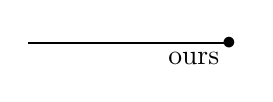
\begin{tikzpicture}[xscale=0.85]
\path (0, 0) coordinate (tip) node{$\bullet$} node[below left]{ours};
\draw (tip) + (-3,0) -- (tip);
\end{tikzpicture}
\\[1em]

(b)
&
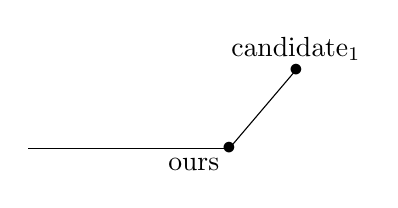
\begin{tikzpicture}[xscale=0.85]
\path (0, 0) coordinate (tip) node{$\bullet$} node[below left]{ours};
\draw (tip) + (-3,0) -- (tip);
\draw (tip) -- ++(1.0,  1.0) node{$\bullet$} coordinate (ab) node[above]{candidate$_1$};
\end{tikzpicture}
&
\begin{tikzpicture}[xscale=0.85]
\path (0, 0) coordinate (tip) node{$\bullet$};
\draw (tip) + (-3,0) -- (tip);
\draw (tip) -- ++(1.0,  1.0) node{$\bullet$} coordinate (ab) node[above]{ours};
\end{tikzpicture}
\\[1em]

(c)
&
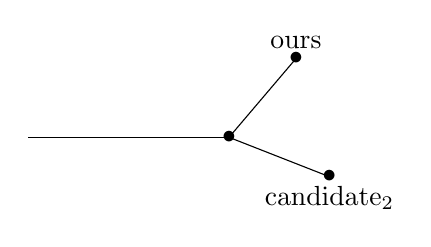
\begin{tikzpicture}[xscale=0.85]
\path (0, 0) coordinate (tip) node{$\bullet$};
\draw (tip) + (-3,0) -- (tip);
\draw (tip) -- ++(1.0,  1.0) node{$\bullet$} coordinate (ab) node[above]{ours};
\draw (tip) -- ++(1.5, -0.5) coordinate (cd) node{$\bullet$} node[below]{candidate$_2$};
\end{tikzpicture}
&
\begin{tikzpicture}[xscale=0.85]
\path (0, 0) coordinate (tip) node{$\bullet$};
\draw (tip) + (-3,0) -- (tip);
\draw (tip) -- ++(1.0,  1.0) node{$\bullet$} coordinate (ab);
\draw (tip) -- ++(1.5, -0.5) coordinate (cd) node{$\bullet$} node[below]{ours};
\end{tikzpicture}
\\[1em]

(d)
&
\begin{tikzpicture}[xscale=0.85]
\path (0, 0) coordinate (tip) node{$\bullet$};
\draw (tip) + (-3,0) -- (tip);
\draw (tip) -- ++(1.0,  1.0) node{$\bullet$} coordinate (ab);
\draw (tip) -- ++(1.5, -0.5) coordinate (cd) node{$\bullet$} node[below]{ours};
\draw (ab) -- ++(0.5,  0.5) -- ++(2.0, 0) node{$\bullet$} node[above]{candidate$_3$};
\end{tikzpicture}
&
\begin{tikzpicture}[xscale=0.85]
\path (0, 0) coordinate (tip) node{$\bullet$};
\draw (tip) + (-3,0) -- (tip);
\draw (tip) -- ++(1.0,  1.0) node{$\bullet$} coordinate (ab);
\draw (tip) -- ++(1.5, -0.5) coordinate (cd) node{$\bullet$};
\draw (ab) -- ++(0.5,  0.5) -- ++(2.0, 0) node{$\bullet$} node[above]{ours};
\end{tikzpicture}
\\[1em]

(e)
&
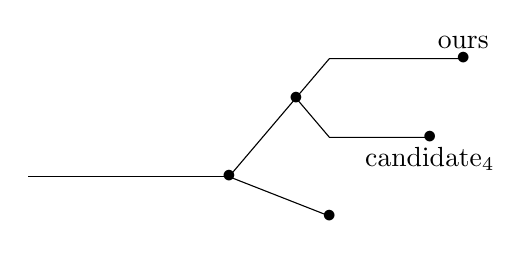
\begin{tikzpicture}[xscale=0.85]
\path (0, 0) coordinate (tip) node{$\bullet$};
\draw (tip) + (-3,0) -- (tip);
\draw (tip) -- ++(1.0,  1.0) node{$\bullet$} coordinate (ab);
\draw (tip) -- ++(1.5, -0.5) coordinate (cd) node{$\bullet$};
\draw (ab) -- ++(0.5,  0.5) -- ++(2.0, 0) node{$\bullet$} node[above]{ours};
\draw (ab) -- ++(0.5, -0.5) -- ++(1.5, 0) node{$\bullet$} node[below]{candidate$_4$};
\end{tikzpicture}
&
\begin{tikzpicture}[xscale=0.85]
\path (0, 0) coordinate (tip) node{$\bullet$};
\draw (tip) + (-3,0) -- (tip);
\draw (tip) -- ++(1.0,  1.0) node{$\bullet$} coordinate (ab);
\draw (tip) -- ++(1.5, -0.5) coordinate (cd) node{$\bullet$};
\draw (ab) -- ++(0.5,  0.5) -- ++(2.0, 0) node{$\bullet$} node[above]{ours};
\draw (ab) -- ++(0.5, -0.5) -- ++(1.5, 0) node{$\bullet$};
\end{tikzpicture}
\\[1em]

(f)
&
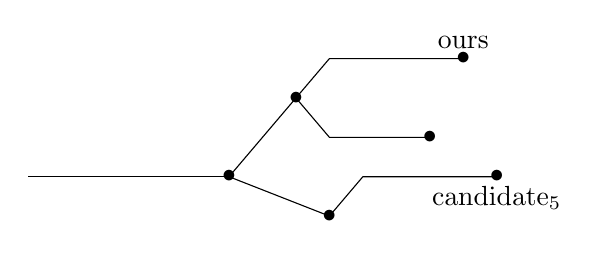
\begin{tikzpicture}[xscale=0.85]
\path (0, 0) coordinate (tip) node{$\bullet$};
\draw (tip) + (-3,0) -- (tip);
\draw (tip) -- ++(1.0,  1.0) node{$\bullet$} coordinate (ab);
\draw (tip) -- ++(1.5, -0.5) coordinate (cd) node{$\bullet$};
\draw (ab) -- ++(0.5,  0.5) -- ++(2.0, 0) node{$\bullet$} node[above]{ours};
\draw (ab) -- ++(0.5, -0.5) -- ++(1.5, 0) node{$\bullet$};
\draw (cd) -- ++(0.5,  0.5) -- ++(2.0, 0) node{$\bullet$} node[below]{candidate$_5$};
\end{tikzpicture}
&
\begin{tikzpicture}[xscale=0.85]
\path (0, 0) coordinate (tip) node{$\bullet$};
\draw (tip) + (-3,0) -- (tip);
\draw (tip) -- ++(1.0,  1.0) node{$\bullet$} coordinate (ab);
\draw (tip) -- ++(1.5, -0.5) coordinate (cd) node{$\bullet$};
\draw (ab) -- ++(0.5,  0.5) -- ++(2.0, 0) node{$\bullet$};
\draw (ab) -- ++(0.5, -0.5) -- ++(1.5, 0) node{$\bullet$};
\draw (cd) -- ++(0.5,  0.5) -- ++(2.0, 0) node{$\bullet$} node[below]{ours};
\end{tikzpicture}
\\
\end{tabular}

\hrule
\caption{\label{normal-chain-evolution}Chain evolution, ``normal'' case}
\end{figure}

\begin{figure}[p]
\hrule

\begin{tabular}{ll@{$\quad\Rightarrow\quad$}l}
a &&
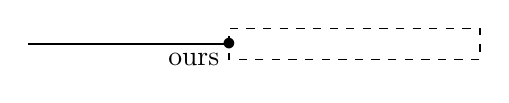
\begin{tikzpicture}[xscale=0.85]
\path (0, 0) coordinate (tip) node{$\bullet$} node[below left]{ours};
\draw [dashed] (tip) -- ++(0, 0.2) -- ++(3.75, 0) -- ++(0, -0.4) -- ++(-3.75, 0) -- cycle;
\draw (tip) + (-3,0) -- (tip);
\end{tikzpicture}
\\

b &&
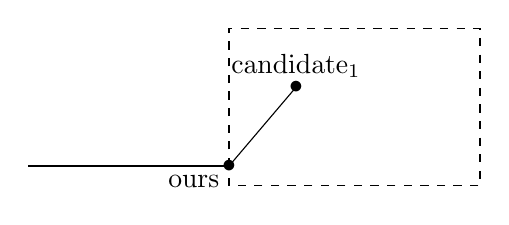
\begin{tikzpicture}[xscale=0.85]
\path (0, 0) coordinate (tip) node{$\bullet$} node[below left]{ours};
\draw [dashed] (tip) -- ++(0, 1.75) -- ++(3.75, 0) -- ++(0, -2) -- ++(-3.75, 0) -- cycle;
\draw (tip) + (-3,0) -- (tip);
\draw (tip) -- ++(1.0,  1.0) node{$\bullet$} coordinate (ab) node[above]{candidate$_1$};
\end{tikzpicture}
\\

c &&
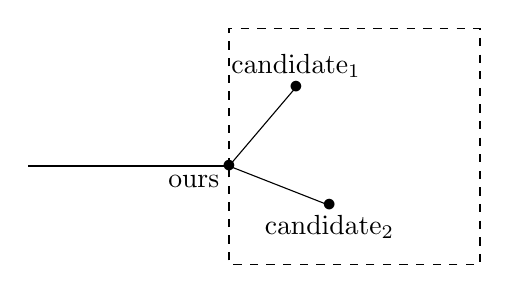
\begin{tikzpicture}[xscale=0.85]
\path (0, 0) coordinate (tip) node{$\bullet$} node[below left]{ours};
\draw [dashed] (tip) -- ++(0, 1.75) -- ++(3.75, 0) -- ++(0, -3) -- ++(-3.75, 0) -- cycle;
\draw (tip) + (-3,0) -- (tip);
\draw (tip) -- ++(1.0,  1.0) node{$\bullet$} coordinate (ab) node[above]{candidate$_1$};
\draw (tip) -- ++(1.5, -0.5) coordinate (cd) node{$\bullet$} node[below]{candidate$_2$};
\end{tikzpicture}
\\

d &&
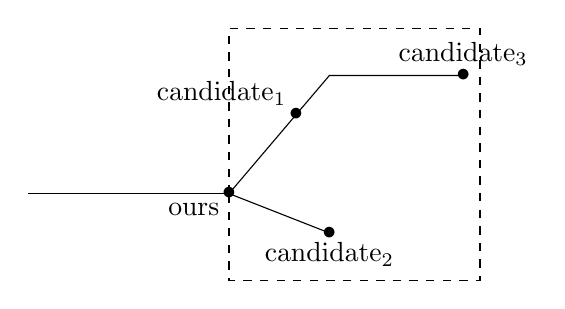
\begin{tikzpicture}[xscale=0.85]
\path (0, 0) coordinate (tip) node{$\bullet$} node[below left]{ours};
\draw [dashed] (tip) -- ++(0, 2.1) -- ++(3.75, 0) -- ++(0, -3.2) -- ++(-3.75, 0) -- cycle;
\draw (tip) + (-3,0) -- (tip);
\draw (tip) -- ++(1.0,  1.0) node{$\bullet$} coordinate (ab) node[above left]{candidate$_1$};
\draw (tip) -- ++(1.5, -0.5) coordinate (cd) node{$\bullet$} node[below]{candidate$_2$};
\draw (ab) -- ++(0.5,  0.5) -- ++(2.0, 0) node{$\bullet$} node[above]{candidate$_3$};
\end{tikzpicture}
\\

e &&
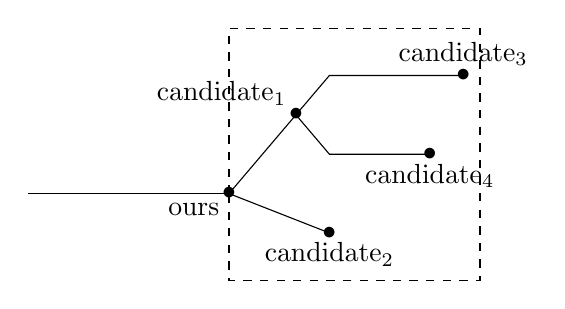
\begin{tikzpicture}[xscale=0.85]
\path (0, 0) coordinate (tip) node{$\bullet$} node[below left]{ours};
\draw [dashed] (tip) -- ++(0, 2.1) -- ++(3.75, 0) -- ++(0, -3.2) -- ++(-3.75, 0) -- cycle;
\draw (tip) + (-3,0) -- (tip);
\draw (tip) -- ++(1.0,  1.0) node{$\bullet$} coordinate (ab) node[above left]{candidate$_1$};
\draw (tip) -- ++(1.5, -0.5) coordinate (cd) node{$\bullet$} node[below]{candidate$_2$};
\draw (ab) -- ++(0.5,  0.5) -- ++(2.0, 0) node{$\bullet$} node[above]{candidate$_3$};
\draw (ab) -- ++(0.5, -0.5) -- ++(1.5, 0) node{$\bullet$} node[below]{candidate$_4$};
\end{tikzpicture}
\\

f &&
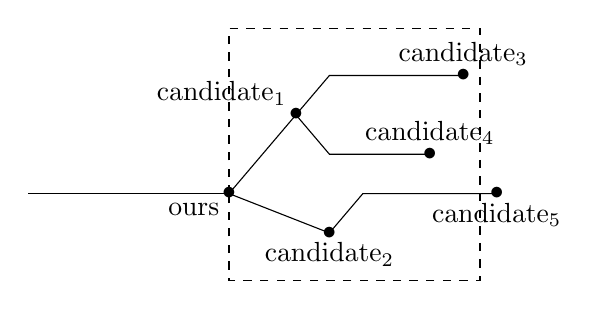
\begin{tikzpicture}[xscale=0.85]
\path (0, 0) coordinate (tip) node{$\bullet$}  node[below left]{ours};
\draw [dashed] (tip) -- ++(0, 2.1) -- ++(3.75, 0) -- ++(0, -3.2) -- ++(-3.75, 0) -- cycle;
\draw (tip) + (-3,0) -- (tip);
\draw (tip) -- ++(1.0,  1.0) node{$\bullet$} coordinate (ab) node[above left]{candidate$_1$};
\draw (tip) -- ++(1.5, -0.5) coordinate (cd) node{$\bullet$} node[below]{candidate$_2$};
\draw (ab) -- ++(0.5,  0.5) -- ++(2.0, 0) node{$\bullet$} node[above]{candidate$_3$};
\draw (ab) -- ++(0.5, -0.5) -- ++(1.5, 0) node{$\bullet$}  node[above]{candidate$_4$};
\draw (cd) -- ++(0.5,  0.5) -- ++(2.0, 0) node{$\bullet$} node[below]{candidate$_5$};
\end{tikzpicture}
\\

g &&
\begin{tikzpicture}[xscale=0.85]
\path (0, 0) coordinate (tip) node{$\bullet$};
\draw [dashed] (tip) -- ++(0, 2.1) -- ++(3.75, 0) -- ++(0, -3.2) -- ++(-3.75, 0) -- cycle;
\draw (tip) + (-3,0) -- (tip);
\draw [dotted] (tip) -- ++(1.0,  1.0) coordinate (ab);
\draw (tip) -- ++(1.5, -0.5) coordinate (cd) node{$\bullet$} node[below]{ours};
\draw [dotted] (ab) -- ++(0.5,  0.5) -- ++(2.0, 0);
\draw [dotted] (ab) -- ++(0.5, -0.5) -- ++(1.5, 0);
\draw (cd) -- ++(0.5,  0.5) -- ++(2.0, 0) node{$\bullet$} node[below]{candidate$_5$};
\end{tikzpicture}
\\

\end{tabular}

\hrule
\caption{\label{delayed-chain-evolution}Chain evolution, ``delay'' case}
\end{figure}

\subsection{Delaying the genesis chain selection rule}

We will now make this intuition precise and apply it to the genesis chain
selection rule. We will rely critically on the following assumption:

\newcommand{\RequiredPeers}{\ensuremath{n_\mathit{rs}}}

\begin{assumption}[Representative sample]
There exists some threshold $\RequiredPeers$ such that if we see the chains of
at least $\RequiredPeers$ peers, we have seen a representative sample of
\emph{all} relevant chains available in the network at that time; there are no
other chains in the network that we do not know about but \emph{should} know
about.
\end{assumption}

This implies that an attacker cannot \emph{eclipse} us; this is something
outside the scope of the consensus layer, and must be guaranteed by the network
layer (probably by a probabilistic way of choosing peers).

Recall that the genesis chain selection rule is designed to help new nodes
connect to the network safely. Indeed, the paper proves \cite[Theorem
2]{cryptoeprint:2018:378} that when a node is up to date, the regular Praos
chain selection rule suffices. We will therefore consider two modes: a
``normal'' mode, to be used when the node is up to date, and the normal
chain selection procedure we have described elsewhere in this document suffices
(\cref{consensus:overview:chainsel,chainsel}), and a ``genesis'' mode in which
we delay chain selection. We will consider how and when we switch between modes
in \cref{genesis:switching-between-modes}; for now, we will assume that we
\emph{are} in genesis mode.

There are two possibilities: either all chains in our window share a common
prefix, or they don't and they fork at the start of the window. We will consider
these two cases separately.

\subsection{Fork: discard}
\label{genesis:discard}

Suppose that $\RequiredPeers = 4$, and our window looks like this:
%
\begin{center}
\begin{tikzpicture}
\path (0, 0) coordinate (tip) node{$\bullet$} node[below left]{tip};
\draw (tip) -- ++(1.0,  1.0) coordinate (ab) node{$\bullet$} node[above left]{$ab$};
\draw [dotted] (tip) -- ++(1.5, -0.5) coordinate (cd);
\draw (ab) -- ++(0.5,  0.5) -- ++(2.0, 0) coordinate(A) node[right]{$A$};
\draw (ab) -- ++(0.5, -0.5) -- ++(2.0, 0) node[right]{$B$};
\draw [dotted] (cd) -- ++(0.5,  0.5) -- ++(1.5, 0) node[right]{$C$};
\draw [dotted] (cd) -- ++(0.5, -0.5) -- ++(1.5, 0) node[right]{$D$};
\draw [dashed]
     (tip)
  -- ++(0, 1.75)
  -- ++(3, 0)
  -- ++(0, -3)
  -- ++(-3, 0) node[pos=0.5, below]{$\underbrace{\hspace{3cm}}_{\text{$s$ slots}}$}
  -- cycle;

%%%%%%%%%%%%%%%%%%%%%%%%%%%%%%%%%%%%%%%%

\draw [red, very thick] (tip) -- (ab) -- ++(0.5,  0.5) -- ++(1.5, 0);
\end{tikzpicture}
\end{center}
%
The thick red line is marking the densest chain section within the window.
Consider what the normal genesis rule would do:
%
\begin{itemize}
\item
Suppose we saw candidate $A$ first, and later discovered $C$ or $D$: since the
intersection between these chains is more than $k$ blocks ago (by assumption),
we would compare the density within a window of $s$ slots from the intersection
point, and then pick the  denser chain. Since that denser chain is $A$, would
stick with $A$.
\item
Conversely, if our current chain was $C$ or $D$, and we would discover $A$,
again the distance from our tip to the intersection point is more than $k$
blocks, and so we would switch to $A$, because $A$ is denser at the intersection
point.
\end{itemize}
%
Either way, we would end up choosing $A$. The window of $s$ slots that is relevant
to distinguish between $A$ and $C$ or $D$ is \emph{precisely} the window we are
currently looking at; this means that we can \emph{discard} candidates $C$
and $D$ at this point; we will never be interested in them. We cannot choose
between $A$ and $B$ yet, because for that we would need to see the window
anchored at the \emph{later} intersection point between those two chains.

\subsection{Common prefix: adopt}
\label{genesis:adopt}

If there is no fork point at the start of the window, then by definition
all candidates must share some common prefix:
%
\begin{center}
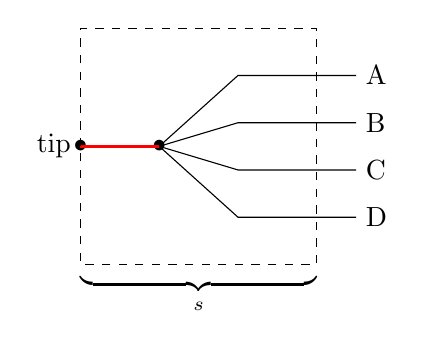
\begin{tikzpicture}
\path (0, 0) coordinate (tip) node{$\bullet$};
\draw (tip) -- ++(1.0,  0.0) coordinate (branch) node{$\bullet$};
\draw (branch) -- ++(1.0,  0.9) -- ++ (1.5, 0) node[right]{A};
\draw (branch) -- ++(1.0,  0.3) -- ++ (1.5, 0) node[right]{B};
\draw (branch) -- ++(1.0, -0.3) -- ++ (1.5, 0) node[right]{C};
\draw (branch) -- ++(1.0, -0.9) -- ++ (1.5, 0) node[right]{D};

%%%%%%%%%%%%%%%%%%%%%%%%%%%%%%%%%%%%%%%%

\node [left] at (tip) {tip};
\draw [red, very thick] (tip) -- ++(1.0,  0.0);
\draw [dashed]
     (tip)
  -- ++(0, 1.5)
  -- ++(3, 0)
  -- ++(0, -3)
  -- ++(-3, 0) node[pos=0.5, below]{$\underbrace{\hspace{3cm}}_s$}
  -- cycle;

\end{tikzpicture}
\end{center}
%
Since by assumption the candidates in our window are a representative sample
of all chains in the network, this means that \emph{all} chains share this
common prefix, and so we can for \emph{sure} adopt those blocks into our
own chain, moving up our window:
%
\begin{center}
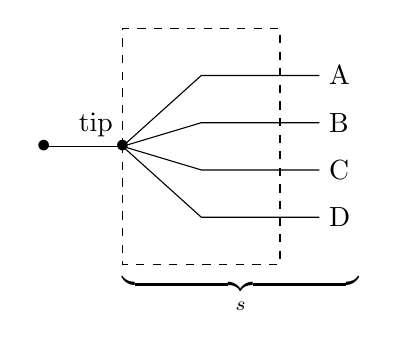
\begin{tikzpicture}
\path (0, 0) coordinate (tip) node{$\bullet$};
\draw (tip) -- ++(1.0,  0.0) coordinate (branch) node{$\bullet$};
\draw (branch) -- ++(1.0,  0.9) -- ++ (1.5, 0) node[right]{A};
\draw (branch) -- ++(1.0,  0.3) -- ++ (1.5, 0) node[right]{B};
\draw (branch) -- ++(1.0, -0.3) -- ++ (1.5, 0) node[right]{C};
\draw (branch) -- ++(1.0, -0.9) -- ++ (1.5, 0) node[right]{D};

%%%%%%%%%%%%%%%%%%%%%%%%%%%%%%%%%%%%%%%%

\node [above left] at (branch) {tip};
\draw [dashed]
     (branch)
  -- ++(0, 1.5)
  -- ++(2, 0)
  -- ++(0, -3)
  -- ++(-2, 0)  node[pos=0.25, below]{$\underbrace{\hspace{3cm}}_s$}
  -- cycle;
\end{tikzpicture}
\end{center}

\subsection{General case}

Notice that we only adopt blocks when they appear on \emph{all} relevant
chains in the system (\cref{genesis:adopt}). This means that we will never have
to roll such blocks back: everything we adopt we are certain about and will
never change our mind about.

This allows us to generalize the pictures from the previous two sections
slightly. Rather than having the window anchored at genesis, it is
anchored at the tip of a chain of blocks that we are sure about; so for the
fork/discard case (\cref{genesis:discard}), the generalization looks like
%
\begin{center}
\begin{tikzpicture}
\path (0, 0) coordinate (tip) node{$\bullet$} node[above left]{tip};
\draw (tip) -- ++(1.0,  1.0) coordinate (ab) node{$\bullet$} node[above left]{$ab$};
\draw [dotted] (tip) -- ++(1.5, -0.5) coordinate (cd);
\draw (ab) -- ++(0.5,  0.5) -- ++(2.0, 0) coordinate(A) node[right]{$A$};
\draw (ab) -- ++(0.5, -0.5) -- ++(2.0, 0) node[right]{$B$};
\draw [dotted] (cd) -- ++(0.5,  0.5) -- ++(1.5, 0) node[right]{$C$};
\draw [dotted] (cd) -- ++(0.5, -0.5) -- ++(1.5, 0) node[right]{$D$};
\draw [dashed]
     (tip)
  -- ++(0, 1.75)
  -- ++(3, 0)
  -- ++(0, -3)
  -- ++(-3, 0) node[pos=0.5, below]{$\underbrace{\hspace{3cm}}_{\text{$s$ slots}}$}
  -- cycle;

%%%%%%%%%%%%%%%%%%%%%%%%%%%%%%%%%%%%%%%%

\draw [red, very thick] (tip) -- (ab) -- ++(0.5,  0.5) -- ++(1.5, 0);
\draw (tip) + (-3,0) node{$\bullet$} -- (tip) node[pos=0.5, below]{$\underbrace{\hspace{3cm}}_\text{immutable}$};
\end{tikzpicture}
\end{center}
%
Similarly, for the common prefix/adopt case (\cref{genesis:adopt}), it looks like
%
\begin{center}
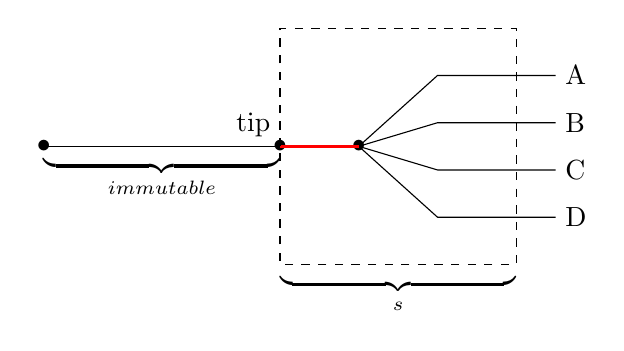
\begin{tikzpicture}
\path (0, 0) coordinate (tip) node{$\bullet$};
\draw (tip) -- ++(1.0,  0.0) coordinate (branch) node{$\bullet$};
\draw (branch) -- ++(1.0,  0.9) -- ++ (1.5, 0) node[right]{A};
\draw (branch) -- ++(1.0,  0.3) -- ++ (1.5, 0) node[right]{B};
\draw (branch) -- ++(1.0, -0.3) -- ++ (1.5, 0) node[right]{C};
\draw (branch) -- ++(1.0, -0.9) -- ++ (1.5, 0) node[right]{D};

%%%%%%%%%%%%%%%%%%%%%%%%%%%%%%%%%%%%%%%%

\node [above left] at (tip) {tip};
\draw [red, very thick] (tip) -- ++(1.0,  0.0);
\draw [dashed]
     (tip)
  -- ++(0, 1.5)
  -- ++(3, 0)
  -- ++(0, -3)
  -- ++(-3, 0) node[pos=0.5, below]{$\underbrace{\hspace{3cm}}_s$}
  -- cycle;
\draw (tip) + (-3,0) node{$\bullet$} -- (tip) node[pos=0.5, below]{$\underbrace{\hspace{3cm}}_\text{immutable}$};

\end{tikzpicture}
\end{center}



\subsection{Switching between modes}
\label{genesis:switching-between-modes}

what if we have to switch back to genesis mode?
(anchor at immutable tip? - yes, Christian confirms.)

\subsection{Notes from meeting with Christian}

emphasize what we mean by mean "by we are closer than s slots from wallclock"

"insufficient blocks": extend dotted line from D
(if D is actually this sort, we can already compare density)

discard based on density
adopt based on common prefix

need tie-breaker: pick arbitrary [should not happen in practice]





\section{Possibly optimizations}

can share validation (20x -> 1x crypto check)
can simplify blockfetch, fewer checks required
  easier to generate longer ranges
  spreading load
bypass volatile DB
if A, B, C, D are all teh same chain, can even just skip ahead<
  ("do you have this point on your chain?")
even more important for genesis, because we need lots of peers
to see all chains
we could support max rollback of 1/4k?
